\documentclass[12pt]{article}
\usepackage{graphicx, caption}

\title{Autocorrelation in Weather}

\author{Rui Zhang}

\date{}

\begin{document}
  \maketitle
  
  \begin{abstract}
    This paper answers whether temperatures of one year are significantly correlated with the next year, across years in a given location, using TAutoCorr.R to calculate correlation and approximately p-value.
  \end{abstract}
  
  \section{Hypothesis}
    Assume one year's temperatures are significantly correlated with the following year's temperatures.
  
  \section{Materials \& Methods}
    Temperatures data is KeyWestAnnualMeanTemperature.Rdata, which is  the temperature in Key West, Florida for 20th century. There are 100 temperature numbers which allow us to get 99 pairs of successive years temperatures.
    
    First, calculate the correlation between these 99 pairs of years temperatures. 
    
    Second, permute the time series randomly and calculate correlation 10000times.
    
    Third, calculate the fraction of correlation coefficients from the second step greater than correlation coefficient calculated in the first step. The fraction is the approximate p-value for the correlation coefficient.
  
  \section{Interpretation}
  The correlation coefficient is 0.3261697, p-value is 2e-04. p-value is small enough for us to give a conclusion that temperatures of one year are significantly correlated with the next year in a given location. Also as Figure 1 showed, one year's temperatures and the following year's temperatures have kind of significant relationship like linear relationship.

  \begin{figure}
    \centering
    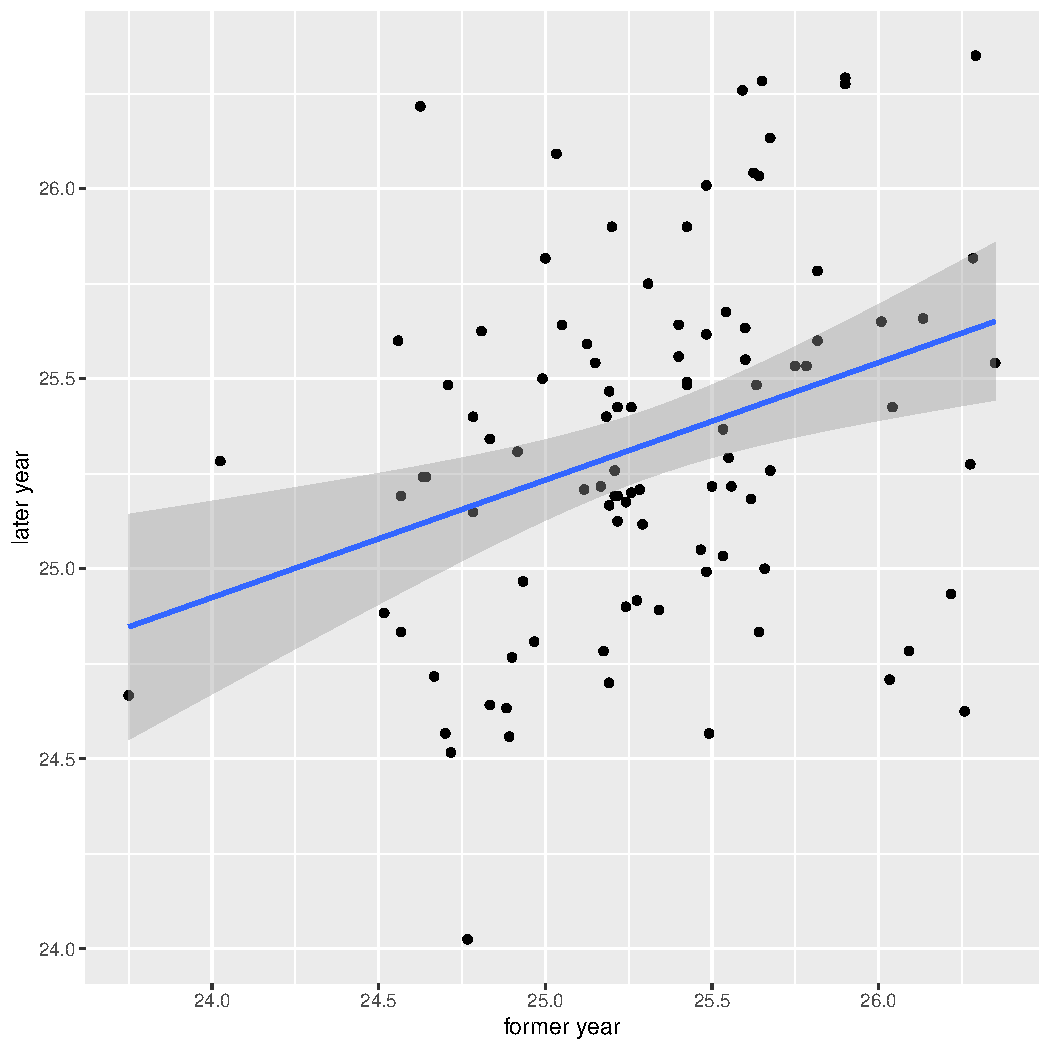
\includegraphics[scale=0.5]{../sandbox/TAutoCorr.pdf}
    \caption{Point plot of paired successive years temperatures}
  \end{figure}
  
\end{document}
